\section{Introduction}\label{sec:intro}

Spatial and immersive audio techniques have been the beneficiaries of
significant research interest over the past few decades.
Recent developments in virtual and augmented reality technologies and
\textit{object-based} audio have led to an acceleration in interest in the
creation of virtual sound fields via approaches such as Wave Field Synthesis
(WFS) and Higher Order Ambisonics (HOA)\cite{berkhout_acoustic_1993,
    ahrens_theory_2008,daniel_further_2003,frank_producing_2015}.
These techniques call for the deployment of large numbers of loudspeakers, and
centralised, \textit{in situ} installations of dedicated hardware and software.
The costs associated with such installations have seen them largely restricted
to the preserve of concert venues, cinemas, and institutions with the means to
purchase and operate large-scale systems of this sort.

Advancements in embedded computing mean that there now exist an assortment of
small, low-cost devices with support for audio digital signal processing (DSP).
These devices are open source, relatively easy to program, and may provide
support for communication over ubiquitous computer networking equipment and
protocols.
A network of such devices could be used to \textit{distribute} the problem of
audio spatialisation, potentially lowering the barrier to entry to what is
otherwise a comparatively exclusive branch of audio research.

The work that this article describes is an exploration of the possibility of
achieving such an outcome.
As such, it is concerned primarily with the transmission of digital audio
signals throughout a computer network.
It is meaningful, then, to reflect on the nature of such signals, a selection
of their properties of greatest pertinence to this work, and the representation
of audio signals within computer systems and networks.

\subsection{Digital Audio Signals}
\label{subsec:digital-audio-signals}

In a digital audio system with sampling rate $F_s$, an audio signal $y$ is
composed of samples $y[n]$, each representing the amplitude of the signal at a
given point in time $t$, where $t = n/F_s$.
For arithmetical convenience, sample amplitudes are typically treated as
floating point numbers, constrained to the interval $y \in [-1, 1]$ (see
\figref{fig:signal-samples}).
It is in this form that audio samples are typically handled during the
processing stage of a DSP algorithm, and the underlying representation
\textemdash{} that required by low level software and hardware systems
\textemdash{} is concealed; matters of numerical resolution and precision are,
by-and-large, abstracted away.

\begin{figure}[ht]
    \centering
    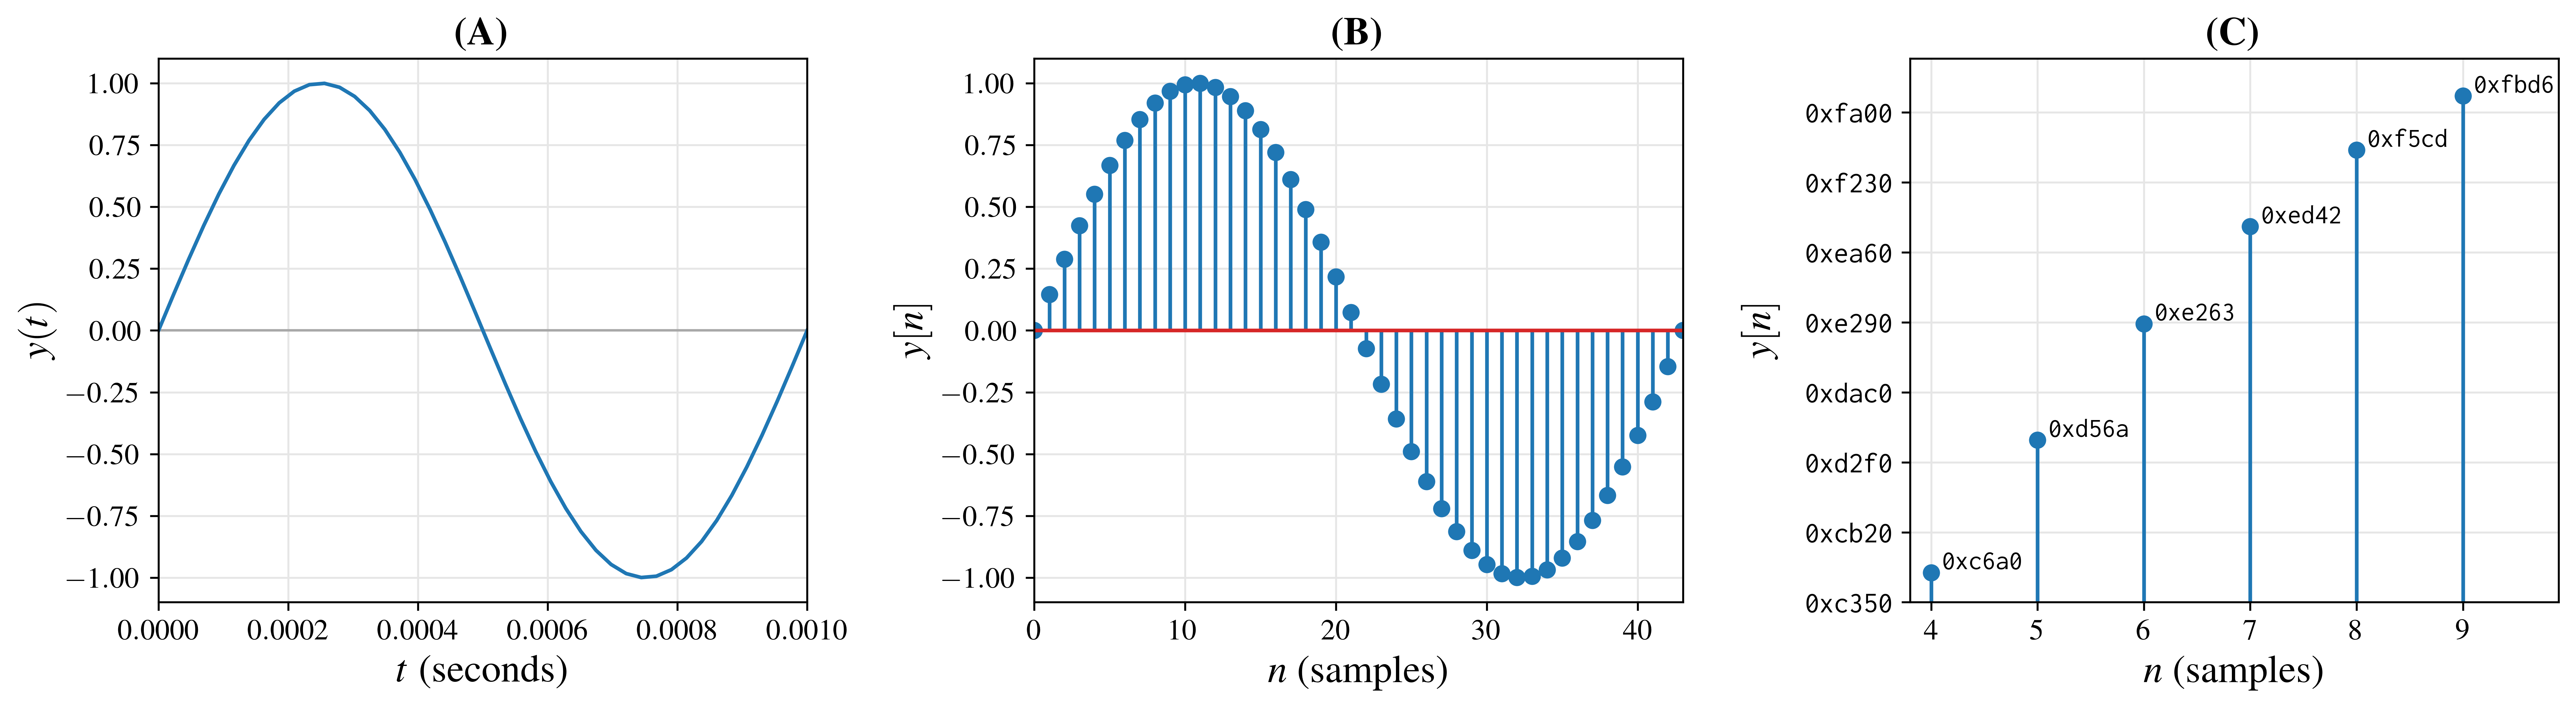
\includegraphics[width=\textwidth]{figures/digital-signal}
    \caption{
        An audio signal (\qty{1}{\kHz} sine wave);
        (a) in continuous time;
        (b) sampled at intervals of $1/Fs$ seconds, with
        $F_s =$~\qty{44.1}{\kHz}.
    }
    \label{fig:signal-samples}
\end{figure}

Samples undergo format conversion at various stages during processing, such as
from an integer pulse code modulation (PCM) filetype to a stream of floating
point audio samples in a digital audio workstation (DAW), or from a floating
point audio stream in an audio device driver to an integer stream to be handled
by a hardware codec.
For the most part, the user, and even the developer of audio software, need not
concern themselves with the rudiments of sample representation and conversion;
as shall be shown, however, under certain circumstances these fundamental
aspects of digital audio systems must be dealt with directly.

\subsection{Numerical Representation}\label{subsec:numerical-representation}

Digital audio samples are ultimately described as streams of binary numbers.
Broadly speaking, the more binary digits (\textit{bits}) available for each
sample, the greater the resolution in terms of distinct amplitudes that can be
represented, with ramifications for dynamic range and signal-to-noise ratio, as
well as for storage and throughput.
Integer sample formats, such as commonly-encountered 16 and 24-bit, offer
comparatively poor resolution at low amplitudes due to the incongruity between
the linear distribution of their values versus the logarithmic nature of sound
intensity.
Floating point formats, by contrast, feature a logarithmic distribution of
available values; the IEEE standard for single-precision (i.e.\ 32-bit) floating
point numbers~\citep{ieee_ieee_1985} dictates that precision is greatest close
to zero, with around half the available values lying in the interval $[-1, 1]$.
To give a brief example, consider the 16-bit case, and a single 16-bit integer
audio sample:
\begin{codelisting}{
        {A 16-bit audio sample, binary representation},
    minted language=text,
    label=listing:binsample
}
    11010101 01101010
\end{codelisting}

\noindent
Separating the bits into two groups of eight is reflective of the fact that the
eight-bit \textit{byte} is typically the unit of transmission in computer
systems.
Grouping the bits in this way points to their expression in hexadecimal format,
transforming the bytes into more easily-digestible morsels of two digits apiece:
\begin{codelisting}{
        {A 16-bit audio sample, hexadecimal representation},
    minted style=bw,
    label=listing:hexsample
}
    d5 6a
\end{codelisting}

\noindent
A number of this kind may also be seen represented (in C and C++ code for
example) as \texttt{0xd56a}, with `\texttt{0x}' indicating that the number to
follow is in base sixteen.
Sixteen bits grant access to $2^{16}=~$65,536 distinct amplitude values for each
sample; what listing~\ref{listing:hexsample} tells us is that, in decimal terms,
this sample should take the 54,634\textsuperscript{th} amplitude
value\footnote{
    For convenience and explicitness elsewhere in the text, decimal equivalents
    to hexadecimal numbers will be indicated with subscript 10, e.g.
    54634\textsubscript{10}.
}.

\subsection{Storage and Transmission}\label{subsec:storage-and-transmission}

Listings~\ref{listing:binsample} and~\ref{listing:hexsample} hint at the
property of \textit{endianness}, i.e.\ the order in which a number's component
bits and bytes appear~\citep{cohen_holy_1981}.
The above representations mirror the left-to-right nature of western written
language and numbers, being \textit{big endian} at the levels of both bit and
byte, with the \textit{most significant bit} (and \textit{most significant
byte}, both abbreviated \textit{MSB}) appearing first.

To paraphrase Cohen~\citep{cohen_holy_1981}, if the unit of digital audio
transmission was \textit{an audio signal}, then endianness would not be a
matter of concern.
Practically speaking, however, to be handled by software or hardware, or
transmitted over a network, audio signals must be decomposed into a hierarchy
of temporally-distributed blocks, those blocks into samples, samples into bytes,
and bytes into bits;
correct endianness must be observed with respect to differing computer
architectures, file formats, and transmission protocols.

The PCM WAV file format, for example, dictates that the least significant byte
of each sample is stored first \textemdash{} little endian \textemdash{} but
that bit order should be big endian~\citep{noauthor_multimedia_1991};
thus the audio sample in listing~\ref{listing:hexsample} should be stored in a
\texttt{.wav} file as \texttt{6ad5}.
The ethernet standard for communication over local area computer
networks~\citep{noauthor_ieee_2018}, by contrast, calls for something akin to
the opposite:
the most significant byte is transmitted first, with each byte sent
little-endian;
returning to the binary representation:
\begin{equation*}
    \texttt{11010101 01101010} \quad\rightarrow\quad \texttt{10101011 01010110}
\end{equation*}
Note, however, that network packet capture software such as
Wireshark\footnote{\url{https://www.wireshark.org/}} reports the bytes of
intercepted packets most significant bit first.


\section{Networked Audio}\label{sec:networked-audio}
\todo[inline]{Less detail on telephony?}
The transmission of audio data has been a topic of research interest since the
earliest days of computer networking as it is recognised today, i.e.\ over
packet-switched networks, whereby data to be transmitted is grouped into packets,
each consisting of a header and a payload.
Voice transmission over ARPANET was being conducted as early as
1974~\citep{schulzrinne_voice_1992} and the first standard for voice
communication over packet-switched networks \textemdash{} the Network Voice
Protocol (NVP) \textemdash{} was released in
1977~\citep{cohen_specifications_1977}.

With its references to `calling' and `ringing', it is clear that the NVP
standard was intended for digital telephony.
Indeed, research on networked audio was primarily concerned with telephony well
into the 1990s, focusing on real-time voice communication over wide area
networks (WAN) with efforts centring on \textit{quality of service} (QoS),
particularly with regard to the perennial issues of latency, packet loss, and
network jitter \textemdash{} inconsistencies in the rate of packet
transmission~\citep{hardman_reliable_1995,hardman_successful_1998}.
Work at this time dealt with streams of compressed audio data, and speech
coding algorithms to overcome the deleterious effects of dropped packets over
unreliable network paths and low-bandwidth connections.

Whereas the priority for digital telephony, and later voice over IP (VoIP)
systems, is intelligibility, for musical purposes fidelity, and the use of
uncompressed audio signals, is of greater concern.
With the increasing availability of high-speed internet connections in the late
1990s came research into transmitting uncompressed audio data over the
internet~\citep{chafe_simplified_2000,xu_real-time_2000}.
Work of this sort was spearheaded by the \textit{SoundWIRE} project, developed
by researchers at McGill University and the Centre for Computer Research in
Music and Acoustics (CCRMA) at Stanford University, and took the form of
a wide variety of experiments with high quality audio over both WAN and local
area networks (LAN).
These experiments included LAN-based real-time musical
performances~\citep{chafe_simplified_2000}, concert streaming over
WAN~\citep{xu_real-time_2000,chafe_simplified_2000}, and sonification of QoS via
a distributed digital waveguide dubbed the
\textit{Network Harp}~\citep{chafe_simplified_2000,chafe_physical_2002}
